\chapter{\ifenglish Background Knowledge and Theory\else ทฤษฎีที่เกี่ยวข้อง\fi}


\section{ด้านโครงสร้างเว็บแอปพลิเคชัน}
ในส่วนนี้จะอธิบายถึงโครงสร้างของเว็บแอปพลิเคชันที่ใช้ในการพัฒนา

\subsection{MVC Architecture}
MVC \cite{web:codebee} เป็นตัวย่อของคำว่า Model View Controller ใช้เรียกรูปแบบการพัฒนาซอฟต์แวร์ที่มีโครงสร้างซึ่งแบ่งออกมาเป็น 3 ส่วนหลัก ตามตัวย่อของชื่อ รูปแบบการพัฒนาซอฟต์แวร์แบบ MVC ถูกนำไปใช้ในขั้นตอนการพัฒนาหลากหลายภาษา
เพราะ MVC เป็นเพียงหลักการออกแบบโปรแกรม (Design Pattern) รูปแบบหนึ่งเท่านั้น ซึ่งเป็นที่นิยมมาก
ในการนำมาพัฒนาแอพพลิเคชั่นซอฟต์แวร์แต่ละแพลตฟอร์ม และประยุกต์ใช้ในอีกหลาย ๆ ด้าน
\subsubsection{ส่วนของ Model (M)}
model คือส่วนของการเก็บรวบรวมข้อมูล ไม่ว่าข้อมูลนั้น ๆ จะถูกจัดเก็บในรูปแบบใดก็ตาม ในฐานข้อมูล
แบบเป็น Object Class หรือที่นิยมเรียกกันว่า VO ( Value Object ) หรือเก็บเป็นไฟล์ข้อมูลเลย
เมื่อข้อมูลถูกโหลดเข้ามาจากที่ต่าง ๆ และเข้ามายังส่วนของโมเดล ตัวโมเดลจะทำการจัดการตระเตรียมข้อมูลให้เป็นรูปแบบที่เหมาะสม เพื่อรอการร้องขอข้อมูลจากส่วนของ Controller
\subsubsection{ส่วนของ View (V)}
view คือส่วนของการแสดงผล หรือส่วนที่จะปฏิสัมพันธ์กับผู้ใช้งาน ( User Interface ) หน้าที่ของ view
ในการเขียนโปรแกรมแบบ MVC คือคอยรับคำสั่งจากส่วนของ Controller และ End User เริ่มแรกเลยตัววิว
อาจจะได้รับคำสั่งจาก Controller ให้แสดงผลหน้า Home และเมื่อผู้ใช้งานหน้าเว็บกดปุ่มสั่งซื้อ View จะส่งข้อมูลไปให้ Controller เพื่อประมวลผลและแสดงบางอย่างจาก Action นั้น
\subsubsection{ส่วนของ Controller (C)}
controller คือส่วนของการเริ่มทำงาน และรับคำสั่ง โดยที่คำสั่งนั้นจะเกิดขึ้นในส่วนการติดต่อกับผู้ใช้งานคือ view
เมื่อผู้ใช้งานทำการ Interactive กับ UI view จะเกิดเหตุการณ์หรือข้อมูลบางอย่างขึ้น ตัววิวจะส่งข้อมูลนั้น
มายัง controller ตัว controller จะทำการประมวลผลโดยบางคำสั่งอาจจะต้องไปติดต่อกับ model ก่อน
เพื่อทำการประมวลผลข้อมูลอย่างถูกต้องเรียบร้อยแล้วก็จะส่งไปยัง view เพื่อแสดงผลตามคำสั่งที่ end user ร้องขอมา
Controller จะทำหน้าที่เป็นตัวกลางระหว่าง Model และ View ให้ทำงานร่วมกันอย่างมีประสิทธิภาพและตรงกับ
ความต้องการของ End User มากที่สุด

\subsection{RESTful API}
RESTful API \cite{web:RESTful} เป็นอินเทอร์เฟซที่ระบบคอมพิวเตอร์สองระบบใช้เพื่อแลกเปลี่ยนข้อมูลผ่านอินเทอร์เน็ตได้อย่างปลอดภัย แอปพลิเคชันทางธุรกิจส่วนใหญ่ต้องสื่อสารกับแอปพลิเคชันภายในอื่นๆ และของบุคคลที่สามเพื่อทำงานต่างๆ ตัวอย่างเช่น หากต้องการสร้างสลิปเงินเดือน ระบบบัญชีภายในของคุณต้องแบ่งปันข้อมูลกับระบบธนาคารของลูกค้าเพื่อออกใบแจ้งหนี้และสื่อสารกับแอปพลิเคชันบันทึกเวลาปฏิบัติงานภายในโดยอัตโนมัติ RESTful API ให้การสนับสนุนการแลกเปลี่ยนข้อมูลนี้เพราะเป็นระบบที่มีมาตรฐานการสื่อสารระหว่างซอฟต์แวร์ที่ปลอดภัย เสถียร และมีประสิทธิภาพ
\subsubsection{API (Application Programming Interface)}
ส่วนต่อประสานโปรแกรมประยุกต์ (Application Programming Interface หรือ API) กำหนดกฎที่คุณต้องปฏิบัติตามเพื่อสื่อสารกับระบบซอฟต์แวร์อื่น โดยนักพัฒนาเปิดเผยหรือสร้าง API เพื่อให้แอปพลิเคชันอื่นสามารถสื่อสารกับแอปพลิเคชันของตนได้ทางโปรแกรม ตัวอย่างเช่น แอปพลิเคชันบันทึกเวลาปฏิบัติงานแสดง API ที่ขอชื่อเต็มของพนักงานและช่วงวันที่ เมื่อได้รับข้อมูลนี้แล้ว ระบบจะประมวลผลบันทึกเวลาปฏิบัติงานของพนักงานเป็นการภายใน และส่งกลับจำนวนชั่วโมงที่ทำงานในช่วงวันที่ดังกล่าว
ทั้งนี้คุณสามารถมองได้ว่า API เว็บเป็นเกตเวย์ระหว่างไคลเอ็นต์และทรัพยากรบนเว็บ

ไคลเอ็นต์
ไคลเอ็นต์คือผู้ใช้ที่ต้องการเข้าถึงข้อมูลจากเว็บ โดยไคลเอ็นต์อาจเป็นบุคคลหรือระบบซอฟต์แวร์ที่ใช้ API ก็ได้ ตัวอย่างเช่น นักพัฒนาสามารถเขียนโปรแกรมที่เข้าถึงข้อมูลสภาพอากาศจากระบบสภาพอากาศ หรือคุณสามารถเข้าถึงข้อมูลเดียวกันจากเบราว์เซอร์เมื่อคุณเยี่ยมชมเว็บไซต์รายงานสภาพอากาศได้โดยตรง

ทรัพยากร
ทรัพยากรคือข้อมูลที่แอปพลิเคชันต่างๆ มอบให้แก่ไคลเอ็นต์ โดยทรัพยากรอาจเป็นรูปภาพ วิดีโอ ข้อความ ตัวเลข หรือข้อมูลประเภทใดก็ได้ ทั้งนี้เครื่องคอมพิวเตอร์ที่มอบทรัพยากรให้แก่ไคลเอ็นต์นั้นเรียกอีกอย่างว่าเซิร์ฟเวอร์ องค์กรต่างๆ ใช้ API เพื่อแบ่งปันทรัพยากรและให้บริการเว็บในขณะที่ยังคงดูแลรักษาความปลอดภัย การควบคุม และการรับรองความถูกต้องไปพร้อมกัน นอกจากนี้ API ยังช่วยให้ลูกค้าระบุได้ว่าไคลเอ็นต์ใดสามารถเข้าถึงทรัพยากรภายในที่เฉพาะเจาะจงได้
\subsubsection{REST (Representational State Transfer)}
REST เป็นสถาปัตยกรรมซอฟต์แวร์ที่กำหนดเงื่อนไขว่า API ควรทำงานอย่างไร โดยแต่แรกเริ่มนั้น มีการสร้าง REST ขึ้นเพื่อเป็นแนวทางในการจัดการการสื่อสารบนเครือข่ายที่ซับซ้อน เช่น อินเทอร์เน็ต คุณสามารถใช้สถาปัตยกรรม REST เพื่อรองรับการสื่อสารที่มีประสิทธิภาพสูงและเชื่อถือได้ในทุกระดับ คุณยังสามารถใช้และปรับเปลี่ยนสถาปัตยกรรมได้อย่างง่ายดาย โดยนำความสามารถในการมองเห็นและการเคลื่อนย้ายข้ามแพลตฟอร์มมาสู่ทุกระบบ API

นักพัฒนา API สามารถออกแบบ API ได้โดยใช้สถาปัตยกรรมต่างๆ โดย API ที่เป็นไปตามรูปแบบสถาปัตยกรรม REST เรียกว่า REST API บริการเว็บที่ใช้สถาปัตยกรรม REST เรียกว่าบริการเว็บ RESTful คำว่า RESTful API โดยทั่วไปหมายถึง API เว็บแบบ RESTful อย่างไรก็ตาม คุณสามารถใช้คำว่า REST API และ RESTful API แทนกันได้
\subsection{ระบบฐานข้อมูล (Database System)}
ระบบฐานข้อมูล (Database System) \cite{web:database} คือ ระบบที่รวบรวมข้อมูลต่าง ๆ ที่เกี่ยวข้องกันเข้าไว้ด้วยกันอย่างมีระบบ มีความสัมพันธ์ระหว่างข้อมูลต่าง ๆ ที่ชัดเจน ในระบบฐานข้อมูลจะประกอบด้วยแฟ้มข้อมูลหลายแฟ้มที่มีข้อมูลเกี่ยวข้องสัมพันธ์กันเข้าไว้ด้วยกันอย่างเป็นระบบและเปิดโอกาสให้ผู้ใช้สามารถใช้งาน
และดูแลรักษาป้องกันข้อมูลเหล่านี้ได้อย่างมีประสิทธิภาพ โดยมีซอฟต์แวร์ที่เปรียบเสมือนสื่อกลางระหว่าง
ผู้ใช้และโปรแกรมต่าง ๆ ที่เกี่ยวข้องกับการใช้ฐานข้อมูล เรียกว่า ระบบจัดการฐานข้อมูล หรือ DBMS (data base management system)มีหน้าที่ช่วยให้ผู้ใช้เข้าถึงข้อมูลได้ง่ายสะดวกและมีประสิทธิภาพ การเข้าถึงข้อมูลของผู้ใช้อาจเป็นการสร้างฐานข้อมูล การแก้ไขฐานข้อมูล หรือการตั้งคำถามเพื่อให้ได้ข้อมูลมา โดยผู้ใช้ไม่จำเป็นต้องรับรู้เกี่ยวกับรายละเอียดภายในโครงสร้างของฐานข้อมูล
\subsubsection{ประโยชน์ของฐานข้อมูล}
\begin{enumerate}
    \item ลดการเก็บข้อมูลที่ซ้ำซ้อน

          ข้อมูลบางชุดที่อยู่ในรูปของแฟ้มข้อมูลอาจมีปรากฏอยู่หลาย ๆ แห่ง เพราะมีผู้ใช้ข้อมูลชุดนี้หลายคน เมื่อใช้ระบบฐานข้อมูลแล้วจะช่วยให้ความซ้ำซ้อนของข้อมูลลดน้อยลง
    \item รักษาความถูกต้องของข้อมูล

          เนื่องจากฐานข้อมูลมีเพียงฐานข้อมูลเดียว ใน
          กรณีที่มีข้อมูลชุดเดียวกันปรากฏอยู่หลายแห่งในฐานข้อมูล ข้อมูลเหล่านี้จะต้องตรงกัน ถ้ามีการแก้ไขข้อมูลนี้ทุก ๆ แห่งที่ข้อมูลปรากฏอยู่จะแก้ไขให้ถูกต้องตามกันหมดโดยอัตโนมัติด้วยระบบจัดการฐานข้อมูล
    \item การป้องกันและรักษาความปลอดภัยให้กับข้อมูลทำได้อย่างสะดวก

          การป้องกันและรักษาความปลอดภัยกับข้อมูลระบบฐานข้อมูลจะให้เฉพาะผู้ที่เกี่ยวข้องเท่านั้น
          ซึ่งก่อให้เกิดความปลอดภัย (security) ของข้อมูลด้วย
\end{enumerate}
\section{ด้านเทคโนโลยี}
ในส่วนนี้จะอธิบายถึงเทคโนโลยีที่ใช้ในการพัฒนาเว็บแอปพลิเคชัน

\subsection{HTML}
HTML \cite{web:html} ย่อมาจาก Hyper Text Markup Language คือภาษาคอมพิวเตอร์ที่ใช้ในการแสดงผลของเอกสารบน website หรือที่เราเรียกกันว่าเว็บเพจ ถูกพัฒนาและกำหนดมาตรฐานโดยองค์กร World Wide Web Consortium (W3C) และจากการพัฒนาทางด้าน Software ของ Microsoft ทำให้ภาษา HTML เป็นอีกภาษาหนึ่งที่ใช้เขียนโปรแกรมได้ หรือที่เรียกว่า HTML Application
HTML เป็นภาษาประเภท Markup สำหรับการการสร้างเว็บเพจ โดยใช้ภาษา HTML สามารถทำโดยใช้โปรแกรม Text Editor ต่างๆ เช่น VS Code, Vim หรือจะอาศัยโปรแกรมที่เป็นเครื่องมือช่วยสร้างเว็บเพจ เช่น Dream Weaver ซึ่งอํานวยความสะดวกในการสร้างหน้า HTML ส่วนการเรียกใช้งานหรือทดสอบการทำงานของเอกสาร HTML จะใช้โปรแกรม web browser เช่น Google Chrome, Microsoft Edge, Mozilla Firefox, Safari และ Opera เป็นต้น
\begin{figure}
    \centering
    
\includegraphics[width=0.5\textwidth]{img/html.png}
    \caption{HTML}
    \label{fig:html}
\end{figure}

\subsection{CSS}
CSS \cite{web:css} ย่อมาจาก Cascading Style Sheet  มักเรียกโดยย่อว่า "สไตล์ชีต" คือภาษาที่ใช้เป็นส่วนของการจัดรูปแบบการแสดงผลเอกสาร  HTML โดยที่ CSS กำหนดกฏเกณฑ์ในการระบุรูปแบบ (หรือ "Style") ของเนื้อหาในเอกสาร อันได้แก่ สีของข้อความ สีพื้นหลัง ประเภทตัวอักษร และการจัดวางข้อความ ซึ่งการกำหนดรูปแบบ หรือ Style นี้ใช้หลักการของการแยกเนื้อหาเอกสาร HTML ออกจากคำสั่งที่ใช้ในการจัดรูปแบบการแสดงผล กำหนดให้รูปแบบของการแสดงผลเอกสาร ไม่ขึ้นอยู่กับเนื้อหาของเอกสาร เพื่อให้ง่ายต่อการจัดรูปแบบการแสดงผลลัพธ์ของเอกสาร HTML โดยเฉพาะในกรณีที่มีการเปลี่ยนแปลงเนื้อหาเอกสารบ่อยครั้ง หรือต้องการควบคุมให้รูปแบบการแสดงผลเอกสาร HTML มีลักษณะของความสม่ำเสมอทั่วกันทุกหน้าเอกสารภายในเว็บไซต์เดียวกัน  โดยกฏเกณฑ์ในการกำหนดรูปแบบ (Style) เอกสาร HTML ถูกเพิ่มเข้ามาครั้งแรกใน HTML 4.0  เมื่อปีพ.ศ. 2539 ในรูปแบบของ CSS level 1 Recommendations ที่กำหนดโดย องค์กร World Wide Web Consortium หรือ W3C
\subsection{TypeScript}
Typescript \cite{web:typescript} คือภาษา JavaScript ใน Version ที่ได้รับการ Upgrade สามารถทำงานบน Node.js Environment หรือ Web Browser ต่าง ๆ ที่มีการรองรับ ECMAScript 3 ขึ้นไป TypeScript เป็น Statically Compiled Language ที่ได้จัดเตรียมทั้ง Static Typing, Classes และ Interface ไว้ให้แล้ว ช่วยให้คุณสามารถเขียน Code ของ JavaScript ที่เรียบง่ายและ Clean ได้อย่างสะดวกขึ้น ดังนั้น การใช้ TypeScript จะช่วยให้คุณสามารถสร้าง Software ที่ปรับใช้งานได้ง่ายและมีประสิทธิภาพมากยิ่งขึ้น

\subsection{Tailwind CSS}
Tailwind CSS \cite{web:tailwind} คือ CSS \cite{web:css} Framework ตัวหนึ่งที่มีรูปแบบการทำงานแบบ Utility-First โดย Utility คือ Class Selector ตัวหนึ่ง ที่เมื่อใช้งานก็เพียงเรียกใช้ Utility ต่างๆมาประกอบกันให้ได้การแสดงผลตามที่เราต้องการ ซึ่งจะมีความต่างกับ CSS Framework อื่นที่มักจะกำหนด Class Selector ให้เฉพาะเจาะจงกับรูปแบบการแสดงผลของ Element นั้น ๆ ไปเลย
\begin{figure}
    \centering
    
\includegraphics[width=0.5\textwidth]{img/tailwind.jpg}
    \caption{Tailwind CSS}
    \label{fig:tailwind}
\end{figure}
\subsection{Next.js}
Next.js \cite{web:nextjs} เป็น open-source React framework ซึ่งต่างจาก React ตรงที่ Next.js เป็นการใช้ server side rendering และยังสามารถทำเว็ปไซต์ได้ทั้งแบบ static และ dynamic ซึ่งข้อดีของการเป็น Server Side Rendering คือ ช่วยในเรื่อง SEO หรือ search engine optimization เพราะถ้าทำการ inspect เว็ปไซต์ที่สร้างโดย Next.js จะเห็นว่า source จะเป็น html ซะส่วนใหญ่ ซึ่งทำให้ SEO ค้นผ่าน source เพื่อให้ได้ข้อมูลและจัดหมวดหมู่ได้ง่ายกว่า React ที่เป็น JavaScript มากกว่า ทำให้ Next.js เป็นที่นิยมในหลาย ๆ บริษัท นอกจากนี้ ข้อดีก็คือ render ได้เร็วกว่า React เพราะ Next.js มีสิ่งที่เรียกว่า get static path ซึ่งการสร้าง path แบบ static แบบเว็ปไซต์ html โดยไม่ต้องทำการเชื่อมต่อกับ back-end เพื่อให้ได้ data ยิ่งไปกว่านั้น Next.js สามารถรวมเข้ากับ back-end ได้ง่ายๆ เพราะ Next.js มีสิ่งที่เรียกว่า API routes ในการรับส่ง request ใน folder ของ page จะมีอีก folder ที่เรียกว่า api ที่ถูกปฏิบัติเป็น endpoint แทนที่จะเป็น page ซึ่ง folder api นี้จะเป็นในส่วนหนึ่งของ server-side เท่านั้น ทำให้ไม่ไปเพิ่ม size ของ Client Side
\begin{figure}
    \centering
    
\includegraphics[width=0.5\textwidth]{img/nextjs.png}
    \caption{Next.js}
    \label{fig:nextjs}
\end{figure}
\subsection{MySQL}
MySQL \cite{web:mysql} คือ ระบบจัดการฐานข้อมูล หรือ Database Management System (DBMS) แบบข้อมูลเชิงสัมพันธ์ หรือ Relational Database Management System (RDBMS) ซึ่งเป็นระบบฐานข้อมูลที่จัดเก็บรวบรวมข้อมูลในรูปแบบตาราง โดยมีการแบ่งข้อมูลออกเป็นแถว (Row) และในแต่ละแถวแบ่งออกเป็นคอลัมน์ (Column) เพื่อเชื่อมโยงระหว่างข้อมูลในตารางกับข้อมูลในคอลัมน์ที่กำหนด แทนการเก็บข้อมูลที่แยกออกจากกัน โดยไม่มีความเชื่อมโยงกัน ซึ่งประกอบด้วยข้อมูล (Attribute) ที่มีความสัมพันธ์เชื่อมโยงกัน (Relation) โดยใช้ RDBMS Tools สำหรับการควบคุมและจัดเก็บฐานข้อมูลที่จำเป็น ทำให้นำไปประยุกต์ใช้งานได้ง่าย ช่วยเพิ่มประสิทธิภาพในการทำงานให้มีความยืดหยุ่นและรวดเร็วได้มากยิ่งขึ้น รวมถึงเชื่อมโยงข้อมูล ที่จัดแบ่งกลุ่มข้อมูลแต่ละประเภทได้ตามต้องการ จึงทำให้ MySQL เป็นโปรแกรมระบบจัดฐานข้อมูลที่ได้รับความนิยมสูง

% \subsection{Docker}

\subsection{JSON}
JSON \cite{web:json} ย่อมาจาก (JavaScript Object Notation) เป็นมาตรฐานในการแลกเปลี่ยนข้อมูล (Data Interchange Format) ที่ได้รับความนิยมแทบจะสูงที่สุดในปัจจุบัน ก่อกำเนิดขึ้นในช่วงต้นยุค 2000 ซึ่ง JSON เป็นที่นิยมโดยเฉพาะในงานด้านการทำ APIs ซึ่งเหล่า developers ทุกคนคงรู้จักและคุ้นเคยกันเป็นอย่างดี แม้ว่าจะมีรูปแบบข้อมูลอื่น ๆ อีกมากมายเช่น XML, CSV, YAML, etc เป็นต้น
\subsubsection{จุดเด่นของ JSON}
\begin{itemize}
    \item อ่านทำความเข้าใจได้ง่าย
    \item มีความเบา (lightweight)
    \item มีความเป็นมาตรฐานสูง และเป็นที่นิยมสูง
    \item มีความเร็วในการ access ข้อมูลที่สูง เพราะไม่ได้มีโครงสร้างที่ซับซ้อนเหมือนเช่น XML เป็นต้น
\end{itemize}


% \subsection{Relational Database Management System (RDBMS)}



\section{ด้าน User Interface}
ในส่วนนี้จะอธิบายถึงการออกแบบ User Interface ของเว็บแอปพลิเคชัน

\subsection{Design Thinking}
กระบวนการออกแบบ design thinking นั้นมีหลากหลายรูปแบบ ทั้งรูปแบบ 3 ขั้น ไปจนถึง 7 ขั้น ทุกรูปแบบมีความคล้ายคลึงมากที่สุด และใช้หลักการเดียวกันที่อ้างอิงจาก Herbert Simon ผู้ชนะรางวัลโนเบลในสาขา The Sciences of the Artificial ในปี 1969 โดยรูปแบบที่นิยมใช้กันมากที่สุด คือ รูปแบบของ Hasso-Plattner Institute of Design at Stanford มีทั้งหมด 5 กระบวนด้วยกัน ดังนี้
\begin{enumerate}
    \item Empathise หรือ การเข้าใจปัญหา
          คือ การทำความเข้าใจกับปัญหาก่อน ตั้งแต่การเข้าใจผู้ใช้ กลุ่มเป้าหมาย หรือเข้าใจสิ่งที่ต้องการแก้ไขเพื่อหาหนทางที่เหมาะสม และดีที่สุดให้ได้ โดยเริ่มต้นจาก การเข้าใจคำถาม สร้างสมมติฐาน กระตุ้นให้เกิดการใช้ความคิดที่นำไปสู่ความคิด สร้างสรรค์ และวิเคราะห์ปัญหาให้ถี่ถ้วน เพื่อหาแนวทางที่ชัดเจน นำไปสู่การแก้ไขปัญหาที่ตรงประเด็น และสร้างผลลัพธ์ที่ดีที่สุด
    \item Define หรือ กำหนดปัญหาให้ชัดเจน
          คือ การเข้าใจความต้องการ ปัญหา และวิเคราะห์ข้อมูลเชิงลึก เพื่อคัดกรองหาปัญหาที่แท้จริง กำหนดหรือบ่งชี้ปัญหาอย่างชัดเจน เพื่อที่จะเป็นแนวทางในการปฎิบัติ และมีทิศทางในการแก้ไขปัญหาอย่างชัดเจน
    \item Ideate หรือ ระดมความคิด
          คือ การนำเสนอแนวคิดต่างๆร่วมกัน ถึงวิธีการแก้ไขปัญหา อย่างไม่มีกรอบจำกัด การระดมความคิดควรมีมุมมองหลากหลาย และมีหลากหลายแนวทางให้ได้มากที่สุด เพื่อให้มีฐานข้อมูลในการนำไปวิเคราะห์และสรุปผล เพื่อนำไปแก้ไขปัญหา โดยไม่จำเป็นต้องเป็นแนวทางใดแนวทางหนึ่ง และการระดมความคิดยังช่วยมองให้เห็นปัญหาที่หลากหลายได้มากขึ้น
    \item Prototype หรือ สร้างต้นแบบที่เลือก
          คือ การออกแบบผลิตภัณฑ์หรือนวัตกรรม เพื่อสร้างต้นแบบสำหรับการทดสอบ และนำไปใช้จริง ซึ่งคือ การลงมือปฎิบัติหรือทดลองตามแนวทางการแก้ไขปัญหาที่ได้กำหนดไว้
    \item Test หรือ ทดสอบการแก้ไขปัญหา นํา Prototype ที่เราทําการทําขึ้นมาไปทดสอบกับผู้ใช้ว่าสามารถแก้ไขปัญหาของ
          ผู้ใช้ได้หรือไม่ และหลังจากนั้นถ้าหากการแก้ปัญหายังไม่สามารถช่วยแก้ไขได้
          หรือแก้ไขได้ยังไม่ดีพอ ผู้จัดทําจะต้องกลับไปทําตั้งแต่ขั้นตอนแรกอีกครั้งจนกว่าจะสามารถออกแบบโปรแกรมที่แก้ไขปัญหา
          ของผู้ใช้ได้


          \begin{figure}
              \begin{center}
                  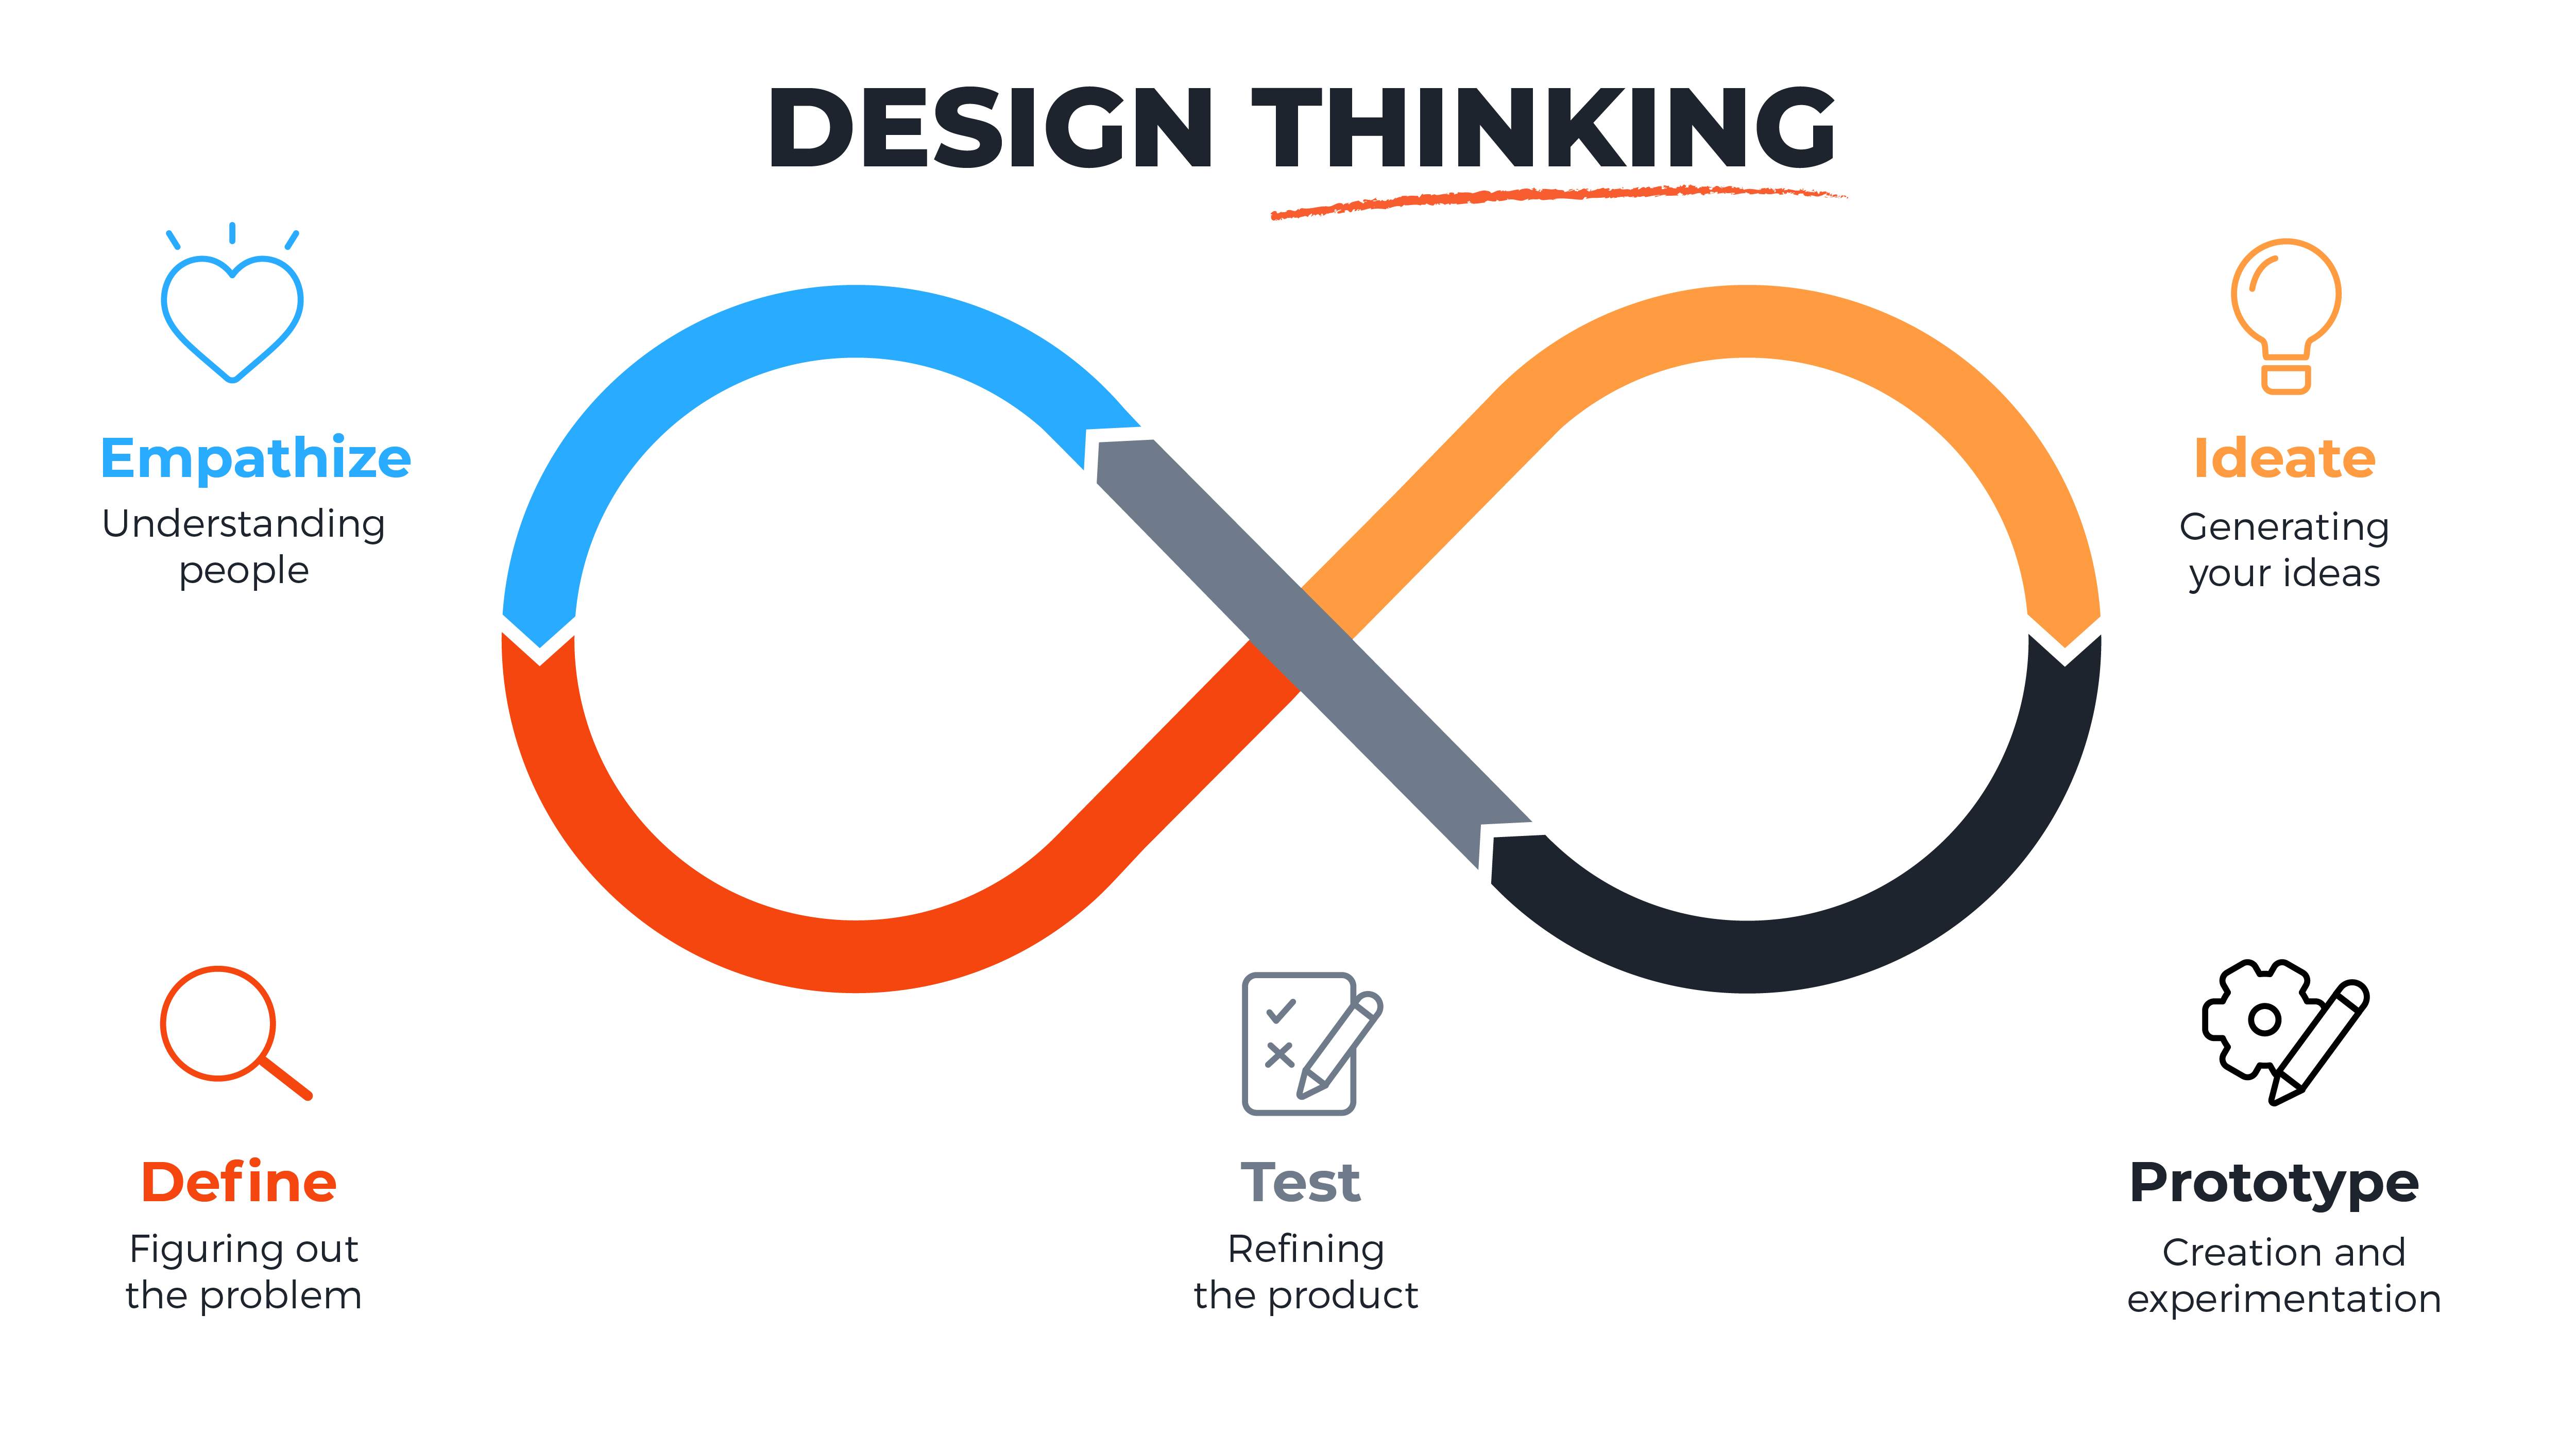
\includegraphics[width=0.8\textwidth]{img/design-thinking.png}
              \end{center}
              \caption[Poem]{กระบวนการออกแบบ Design Thinking}
              \label{fig:design-thinking}
          \end{figure}

\end{enumerate}


% \noindent
% where $\omega$ is the frequency of the plasmon, $c$ is the speed of
% light, $\varepsilon_m$ is the dielectric constant of the metal,
% $\varepsilon_i$ is the dielectric constant of neighboring insulator,
% and $\varepsilon_\mathit{air}$ is the dielectric constant of air.

% \section{About using figures in your report}

% % define a command that produces some filler text, the lorem ipsum.
% \newcommand{\loremipsum}{
%   \textit{Lorem ipsum dolor sit amet, consectetur adipisicing elit, sed do
%   eiusmod tempor incididunt ut labore et dolore magna aliqua. Ut enim ad
%   minim veniam, quis nostrud exercitation ullamco laboris nisi ut
%   aliquip ex ea commodo consequat. Duis aute irure dolor in
%   reprehenderit in voluptate velit esse cillum dolore eu fugiat nulla
%   pariatur. Excepteur sint occaecat cupidatat non proident, sunt in
%   culpa qui officia deserunt mollit anim id est laborum.}\par}

% \begin{figure}
%   \centering

%   \fbox{
%      \parbox{.6\textwidth}{\loremipsum}
%   }

%   % To include an image in the figure, say myimage.pdf, you could use
%   % the following code. Look up the documentation for the package
%   % graphicx for more information.
%   % \includegraphics[width=\textwidth]{myimage}

%   \caption[Sample figure]{This figure is a sample containing \gls{lorem ipsum},
%   showing you how you can include figures and glossary in your report.
%   You can specify a shorter caption that will appear in the List of Figures.}
%   \label{fig:sample-figure}
% \end{figure}

% Using \verb.\label. and \verb.\ref. commands allows us to refer to
% figures easily. If we can refer to Figures
% \ref{fig:walrus} and \ref{fig:sample-figure} by name in the {\LaTeX}
% source code, then we will not need to update the code that refers to it
% even if the placement or ordering of the figures changes.

% \loremipsum\loremipsum

% % This code demonstrates how to get a landscape table or figure. It
% % uses the package lscape to turn everything but the page number into
% % landscape orientation. Everything should be included within an
% % \afterpage{ .... } to avoid causing a page break too early.
% \afterpage{
%   \begin{landscape}
%   \begin{table}
%     \caption{Sample landscape table}
%     \label{tab:sample-table}

%     \centering

%     \begin{tabular}{c||c|c}
%         Year & A & B \\
%         \hline\hline
%         1989 & 12 & 23 \\
%         1990 & 4 & 9 \\
%         1991 & 3 & 6 \\
%     \end{tabular}
%   \end{table}
%   \end{landscape}
% }

% \loremipsum\loremipsum\loremipsum

% \section{Overfull hbox}

% When the \verb.semifinal. option is passed to the \verb.cpecmu. document class,
% any line that is longer than the line width, i.e., an overfull hbox, will be
% highlighted with a black solid rule:
% \begin{center}
% \begin{minipage}{2em}
% juxtaposition
% \end{minipage}
% \end{center}

\section{\ifenglish%
      \ifcpe CPE \else ISNE \fi knowledge used, applied, or integrated in this project
  \else%
      ความรู้ตามหลักสูตรซึ่งถูกนำมาใช้หรือบูรณาการในโครงงาน
  \fi
 }

\begin{itemize}
    \item 261207 Basic CPE Lab นําความรู้ทางด้าน HTML, CSS, JavaScript และ React.JS รวมถึง
          Node.js ทั้งด้านของ front-end ที่แสดงผลผ่านเว็บไซต์ และ back-end ที่เชื่อมต่อกับฐานข้อมูล
    \item 261361 Software Engineering การใช้กระบวนการทางวิศวกรรมในการดูแลการผลิต ตั้งแต่การเริ่ม
          เก็บความต้องการ การตั้งเป้าหมายของระบบ การออกแบบ กระบวนการพัฒนา การตรวจสอบ การประเมิน
          ผล และทดสอบระบบ
    \item 261342 Database Systems การนําข้อมูลมาเก็บในรูปแบบตาราง การทํา UML และการออกแบบ ER
          diagrams ของเว็บแอพพลิเคชั่นที่จะทํา

          % \item 261102 Computer Programming การเขียน ทดสอบ และดูแลซอร์สโค้ดของโปรแกรมคอมพิวเตอร์
          %       ซึ่งซอร์สโค้ดนั้นจะเขียนด้วยภาษาโปรแกรม ขั้นตอนการเขียนโปรแกรมต้องการความรู้ในหลายด้านด้วยกัน
          %       รวมถึงการนํา GitHub มาใช้ในการเขียนโปรแกรม
\end{itemize}

% อธิบายถึงความรู้ และแนวทางการนำความรู้ต่างๆ ที่ได้เรียนตามหลักสูตร ซึ่งถูกนำมาใช้ในโครงงาน

\section{\ifenglish%
      Extracurricular knowledge used, applied, or integrated in this project
  \else%
      ความรู้นอกหลักสูตรซึ่งถูกนำมาใช้หรือบูรณาการในโครงงาน
  \fi
 }

% อธิบายถึงความรู้ต่างๆ ที่เรียนรู้ด้วยตนเอง และแนวทางการนำความรู้เหล่านั้นมาใช้ในโครงงาน
